\documentclass[11pt]{article}

\usepackage[brazilian]{babel}
\usepackage[utf8]{inputenc}
\usepackage[T1]{fontenc}

\usepackage{graphicx}
\usepackage{subfig}

\usepackage{amsmath}
\usepackage{algorithm}
\usepackage[noend]{algpseudocode}

\title{\textbf{Algoritmo Genético - Problema da Mochila}}

\author{André Minoro Fusioka}

\date{}
\begin{document}

\maketitle

\section{Penalização}

Para a penalização de indivíduos da populção avaliada, foi adotada a seguinte métrica: 
$$
fitness\_ajustado(x_n) =
\begin{cases}
 fitness(x_n) & \text{ se } peso(x_n) \leq  C \\ 
 \frac{1}{peso(x_n)} & \text{ se } peso(x_n) >  C 
\end{cases}
$$
onde $fitness\_ajustado$ é o valor do fitness após a penalização, os valores mais altos são selecionados para a próxima geração. O $peso(x_n)$ é a soma do peso de todos os itens na mochila do n-ésimo indivíduo. Desse modo, quanto maior o peso da mochila de um individuo, menor o fitness e por consequência são menores as chances de ser selecionado  para a próxima geração.

O código abaixo ilustra o cálculo:

\begin{algorithm}
	\caption{Fitness Ajustada}\label{euclid}
	\begin{algorithmic}[1]
		\Function{FitnessAjustada}{população}
		
			\State $fitness\_ajustado \gets []$
			
			\Loop { $\forall$ $individuo$ da $população$:}
				 \State $peso \gets calcular\_peso(individuo)$
				\If{$peso < C$}
				
					\State $fitness \gets calcular\_fitness(individuo) $
				 \Else
					\State $fitness \gets \frac{1}{peso}$		 
				\EndIf
				\State \textbf{adicione} o $fitness$ à lista $fitness\_ajustado$
			\EndLoop {\textbf{end loop}}
			\State \Return $fitness\_ajustado$
		\EndFunction
	\end{algorithmic}
\end{algorithm}

Cada indivíduo tem o seu peso calculado, se estiver abaixo do limite o fitness real é adicionado à lista de fitness ajustado (sem realizar operação nenhuma), caso esteja acima do limite o fitness penalizado será calculado conforme descrito e então adicionado à lista de fintess ajustado. 

\section{Reparação}

Para a reparação o peso de cada mochila de cada indivíduo é avaliado e enquanto for maior que o limite um item aleatório é retirado. Quando o peso estiver dentro do limite o fitness dessa mochila é avaliada e adicionada a lista de fintess reparada. O pseudocódigo é exibido abaixo: 


\begin{algorithm}
	\caption{Fitness Reparado}\label{euclid}
	\begin{algorithmic}[1]
		\Function{FitnessReparado}{população}
		
			\State $fitness\_reparado \gets []$
			
			\Loop{ $\forall$ $individuo$ da $população$:}
				\State $peso \gets calcular\_peso(individuo)$
				
				\Loop{ \textbf{enquanto} $peso$ > $C$}
					\State $ individuo \gets remove\_item\_aleatorio(individuo) $
					\State $peso \gets calcular\_peso(individuo)$
				\EndLoop{\textbf{end loop}}
				
				
				\State \textbf{adicione} o $fitness$ à lista $fitness\_reparado$
			\EndLoop{\textbf{end loop}}
			\State \Return $fitness\_reparado$
		\EndFunction
	\end{algorithmic}
\end{algorithm}

Dessa forma, caso os itens da mochila do indivíduo estejam dentro do limite permitido seu fitness é adicionado à lista de fintess reparados (sem realizar operação nenhuma), caso esteja acima do limite um item aleatório é removido da mochila até estar dentro do limite, quando estiver dentro do limite seu fitness é calculado e adicionado à solução.

\section{Penalização x Reparação}

A figura \ref{fig:ag_comparacao_500_500_09_01} exibe um exemplo da comparação das abordagens de desenvolvimento em que o tamanho da população  ($Np = 500$) é igual ao número de gerações, com uma probabilidade de crossover de $Pc = 90\%$ e $Pm = 10\%$ de mutação. A curva vermelha represanta a penalização e a azul a reparação.

A figura \ref{fig:comparacao_500_500_08_005} exibe os resultados para $Np = 500$ e gerações igual ao número de gerações, com $ Pm = 80\% $ e $Pc = 5\%$.


A figura \ref{fig:comparacao_populacao_menor_geracao} exibe o gráfico para tamanho da população  ($Np = 100$) \textbf{inferior} ao número de gerações ($Ng = 500$). A figura \ref{fig:comparacao_100_500_09_01} representa uma configuração com $Pc = 90\%$ e $Pm = 10\% $ e a figura \ref{fig:comparacao_100_500_08_005} ilustra $Pc = 80\%$ e $ Pm = 5\%$ de mutação.

\begin{figure}[h]
	\centering
	\subfloat[Np=500 Pc=90\% Pm=10\%]{
		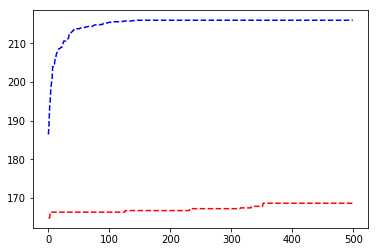
\includegraphics[scale=0.4]{ag_comparacao_500_500_09_01.png}
		\label{fig:ag_comparacao_500_500_09_01}
	}
	\quad %espaco separador
	\subfloat[Np=500 Pc=80\% Pm=5\%]{
		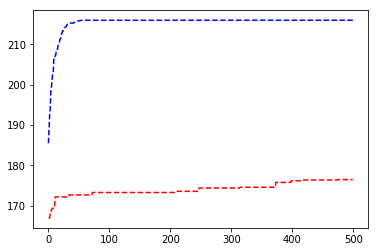
\includegraphics[scale=0.4]{ag_comparacao_500_500_08_005.png}
		\label{fig:comparacao_500_500_08_005}
	}
	\caption{Gráficos de comparação entre as abordagens de penalização e reparação com população \textbf{igual} ao número de gerações}
	\label{fig:comparacao_populacao_igual_geracao}
\end{figure}


\begin{figure}[!h]
	\centering
	\subfloat[Np=100 Ng=500 Pc=90\% Pm=10\%]{
		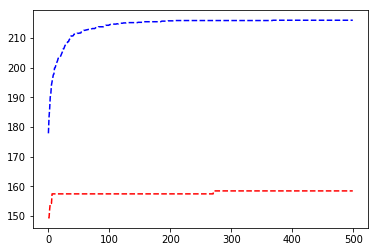
\includegraphics[scale=0.4]{ag_comparacao_100_500_09_01.png}
		\label{fig:comparacao_100_500_09_01}
	}
	\quad %espaco separador
	\subfloat[Np=100 Ng=500 Pc=80\% Pm=5\%]{
		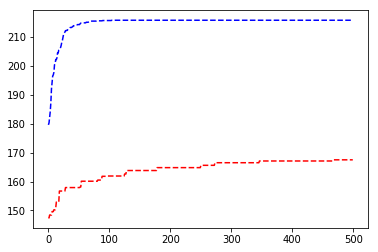
\includegraphics[scale=0.4]{ag_comparacao_100_500_08_005.png}
		\label{fig:comparacao_100_500_08_005}
	}
	\caption{Gráficos de comparação entre as abordagens de penalização e reparação com população \textbf{menor} que o número de gerações}
	\label{fig:comparacao_populacao_menor_geracao}
\end{figure}



Em todos os casos o comportamento a reparação se mostrou superior, enquanto subindo rápidamente para um valor ótimo, enquanto a penalização teve um crescimento mais lento, com uma melhora lenta e inferior à reparação.

Para a reparação nota-se um crescimento rápido nas primeiras gerações e então uma estabilização na solução ótima, enquanto para a penalização possuí um leve crescimento durante as gerações com alguns crescimentos mais abruptos dando o comportamento de "degrau" à curva.

A vantagem da reparação é não permitir que indivíduos não factíveis passem para as próximas gerações, sempre havendo uma melhora (ou estabilização) de uma geração para a outra. Enquanto que o uso penalização pode haver indivíduos não factíveis, principalmente nas primeiras gerações. Então, caso haja uma inicialização ruim (com muitos indivíduos infactíveis) pode haver uma demora maior para a melhora das soluções.

\section{Soluções encontradas}

Todos os testes foram executados dez vezes, com um número máximo de 500 gerações. O número de mochilas apresentados leva em consideração todas as execuções. Nessa seção só será exibida uma mochila devido o tamanho da saída.

Abordagem: Penalização; Tamanho População (Np): 500; P. Crossover (Pc): 90\%; P. Mutação (Pm): 10\% 

Executando o algoritmo dez vezes obteve-se um total de 496 mochilas com valor igual a melhor solução. Exemplos de mochila:

\texttt{
	< 19, 118.000000, 179.000000, 0, 0, 0, 1, 0, 1, 1, 1, 1, 0, 0, 0, 0, 1, 1, 0, 0, 0, 1, 0, 1, 1, 1, 1, 0, 0, 1, 1, 1, 0, 0, 0, 0, 1, 0, 0, 0, 1, 0, 0, 1, 1 > 

%< 19, 118.000000, 179.000000, 0, 0, 0, 1, 0, 1, 1, 1, 1, 0, 0, 0, 0, 1, 1, 0, 0, 0, 1, 0, 1, 1, 1, 1, 0, 0, 1, 1, 1, 0, 0, 0, 0, 1, 0, 0, 0, 1, 0, 0, 1, 1 > 

%< 19, 118.000000, 179.000000, 0, 0, 0, 1, 0, 1, 1, 1, 1, 0, 0, 0, 0, 1, 1, 0, 0, 0, 1, 0, 1, 1, 1, 1, 0, 0, 1, 1, 1, 0, 0, 0, 0, 1, 0, 0, 0, 1, 0, 0, 1, 1 > 

}




\bigbreak




Abordagem: Reparação; Tamanho População (Np): 500; Máximo gerações: 500; P. Crossover (Pc): 90\%; P. Mutação (Pm): 10\% 

Executando o algoritmo dez vezes obteve-se um total de 3936 mochilas com valor igual a melhor solução. Exemplos de mochila:

\texttt{
	< 14, 120.000000, 216.000000, 0, 0, 0, 1, 0, 0, 0, 0, 1, 1, 0, 0, 0, 0, 1, 0, 0, 1, 1, 0, 0, 1, 0, 1, 0, 0, 0, 0, 1, 1, 0, 0, 0, 1, 0, 0, 0, 1, 0, 1, 0, 1 > 

< 14, 120.000000, 216.000000, 0, 0, 0, 1, 0, 0, 0, 0, 1, 1, 0, 0, 0, 0, 1, 0, 0, 1, 1, 0, 0, 1, 0, 1, 0, 0, 0, 0, 1, 1, 0, 0, 0, 1, 0, 0, 0, 1, 0, 1, 0, 1 > 

< 14, 120.000000, 216.000000, 0, 0, 0, 1, 0, 0, 0, 0, 1, 1, 0, 0, 0, 0, 1, 0, 0, 1, 1, 0, 0, 1, 0, 1, 0, 0, 0, 0, 1, 1, 0, 0, 0, 1, 0, 0, 0, 1, 0, 1, 0, 1 > 
}


\bigbreak


Abordagem: Penalização; Tamanho População (Np): 500; Máximo gerações: 500; P. Crossover (Pc): 80\%; P. Mutação (Pm): 50\% 

Executando o algoritmo dez vezes obteve-se um total de 499 mochilas com valor igual a melhor solução. Exemplos de mochila:

\texttt{
	< 14, 114.000000, 186.000000, 0, 0, 0, 0, 0, 0, 1, 0, 1, 1, 0, 1, 0, 0, 0, 0, 0, 1, 1, 0, 0, 0, 0, 0, 1, 0, 0, 1, 1, 1, 0, 0, 0, 1, 1, 0, 0, 1, 0, 0, 0, 1 > 

< 14, 114.000000, 186.000000, 0, 0, 0, 0, 0, 0, 1, 0, 1, 1, 0, 1, 0, 0, 0, 0, 0, 1, 1, 0, 0, 0, 0, 0, 1, 0, 0, 1, 1, 1, 0, 0, 0, 1, 1, 0, 0, 1, 0, 0, 0, 1 > 

< 14, 114.000000, 186.000000, 0, 0, 0, 0, 0, 0, 1, 0, 1, 1, 0, 1, 0, 0, 0, 0, 0, 1, 1, 0, 0, 0, 0, 0, 1, 0, 0, 1, 1, 1, 0, 0, 0, 1, 1, 0, 0, 1, 0, 0, 0, 1 > 
}

\bigbreak



Abordagem: Reparação; Tamanho População (Np): 500; Máximo gerações: 500; P. Crossover (Pc): 80\%; P. Mutação (Pm): 50\% 

Executando o algoritmo dez vezes obteve-se um total de 4584 mochilas com valor igual a melhor solução. Exemplos de mochila:

\texttt{
	< 13, 120.000000, 216.000000, 0, 0, 0, 1, 0, 0, 0, 1, 1, 1, 0, 0, 0, 0, 1, 0, 0, 1, 1, 0, 0, 0, 0, 0, 0, 0, 0, 0, 1, 1, 0, 0, 0, 1, 0, 0, 0, 1, 0, 1, 0, 1 > 

< 13, 120.000000, 216.000000, 0, 0, 0, 1, 0, 0, 0, 1, 1, 1, 0, 0, 0, 0, 1, 0, 0, 1, 1, 0, 0, 0, 0, 0, 0, 0, 0, 0, 1, 1, 0, 0, 0, 1, 0, 0, 0, 1, 0, 1, 0, 1 > 

< 13, 120.000000, 216.000000, 0, 0, 0, 1, 0, 0, 0, 1, 1, 1, 0, 0, 0, 0, 1, 0, 0, 1, 1, 0, 0, 0, 0, 0, 0, 0, 0, 0, 1, 1, 0, 0, 0, 1, 0, 0, 0, 1, 0, 1, 0, 1 > 
}

\bigbreak



Abordagem: Penalização; Tamanho População (Np): 100; Máximo gerações: 500; P. Crossover (Pc): 90\%; P. Mutação (Pm): 10\% 

Executando o algoritmo dez vezes obteve-se um total de 993 mochilas com valor igual a melhor. Exemplos de mochila:

\texttt{
	< 14, 117.000000, 173.000000, 0, 0, 0, 0, 0, 1, 1, 1, 1, 0, 0, 0, 0, 0, 1, 0, 0, 1, 1, 0, 0, 0, 0, 0, 0, 0, 0, 1, 0, 0, 0, 0, 1, 1, 0, 1, 0, 1, 0, 0, 1, 1 > 

< 14, 117.000000, 173.000000, 0, 0, 0, 0, 0, 1, 1, 1, 1, 0, 0, 0, 0, 0, 1, 0, 0, 1, 1, 0, 0, 0, 0, 0, 0, 0, 0, 1, 0, 0, 0, 0, 1, 1, 0, 1, 0, 1, 0, 0, 1, 1 > 

< 14, 117.000000, 173.000000, 0, 0, 0, 0, 0, 1, 1, 1, 1, 0, 0, 0, 0, 0, 1, 0, 0, 1, 1, 0, 0, 0, 0, 0, 0, 0, 0, 1, 0, 0, 0, 0, 1, 1, 0, 1, 0, 1, 0, 0, 1, 1 > 
}

\bigbreak




Abordagem: Reparação; Tamanho População (Np): 100; Máximo gerações: 500; P. Crossover (Pc): 90\%; P. Mutação (Pm): 10\% 

Executando o algoritmo dez vezes obteve-se um total de 3312 mochilas com valor igual a melhor. Exemplos de mochila:

\texttt{
	< 13, 120.000000, 216.000000, 0, 0, 0, 1, 0, 0, 0, 1, 1, 1, 0, 0, 0, 0, 1, 0, 0, 1, 1, 0, 0, 0, 0, 0, 0, 0, 0, 0, 1, 1, 0, 0, 0, 1, 0, 0, 0, 1, 0, 1, 0, 1 > 

< 13, 120.000000, 216.000000, 0, 0, 0, 1, 0, 0, 0, 1, 1, 1, 0, 0, 0, 0, 1, 0, 0, 1, 1, 0, 0, 0, 0, 0, 0, 0, 0, 0, 1, 1, 0, 0, 0, 1, 0, 0, 0, 1, 0, 1, 0, 1 > 

< 13, 120.000000, 216.000000, 0, 0, 0, 1, 0, 0, 0, 1, 1, 1, 0, 0, 0, 0, 1, 0, 0, 1, 1, 0, 0, 0, 0, 0, 0, 0, 0, 0, 1, 1, 0, 0, 0, 1, 0, 0, 0, 1, 0, 1, 0, 1 > 
}



\bigbreak

Abordagem: Penalização; Tamanho População (Np): 100; Máximo gerações: 500; P. Crossover (Pc): 80\%; P. Mutação (Pm): 5\% 

Executando o algoritmo dez vezes obteve-se um total de 418 mochilas com valor igual a melhor. Exemplos de mochila:

\texttt{
	< 16, 117.000000, 175.000000, 1, 0, 0, 1, 0, 1, 0, 1, 0, 1, 0, 0, 1, 0, 0, 1, 0, 1, 1, 1, 0, 0, 0, 0, 1, 0, 0, 0, 1, 0, 0, 0, 1, 0, 1, 0, 0, 0, 0, 1, 0, 1 > 

%< 16, 117.000000, 175.000000, 1, 0, 0, 1, 0, 1, 0, 1, 0, 1, 0, 0, 1, 0, 0, 1, 0, 1, 1, 1, 0, 0, 0, 0, 1, 0, 0, 0, 1, 0, 0, 0, 1, 0, 1, 0, 0, 0, 0, 1, 0, 1 > 

%< 16, 117.000000, 175.000000, 1, 0, 0, 1, 0, 1, 0, 1, 0, 1, 0, 0, 1, 0, 0, 1, 0, 1, 1, 1, 0, 0, 0, 0, 1, 0, 0, 0, 1, 0, 0, 0, 1, 0, 1, 0, 0, 0, 0, 1, 0, 1 > 
}

\bigbreak



Abordagem: Reparação; Tamanho População (Np): 100; Máximo gerações: 500; P. Crossover (Pc): 80\%; P. Mutação (Pm): 5\% 

Executando o algoritmo dez vezes obteve-se um total de 3946 mochilas com valor igual a melhor. Exemplos de mochila:

\texttt{
	< 13, 120.000000, 216.000000, 0, 0, 0, 1, 0, 0, 0, 1, 1, 1, 0, 0, 0, 0, 1, 0, 0, 1, 1, 0, 0, 0, 0, 0, 0, 0, 0, 0, 1, 1, 0, 0, 0, 1, 0, 0, 0, 1, 0, 1, 0, 1 > 

< 13, 120.000000, 216.000000, 0, 0, 0, 1, 0, 0, 0, 1, 1, 1, 0, 0, 0, 0, 1, 0, 0, 1, 1, 0, 0, 0, 0, 0, 0, 0, 0, 0, 1, 1, 0, 0, 0, 1, 0, 0, 0, 1, 0, 1, 0, 1 > 

< 13, 120.000000, 216.000000, 0, 0, 0, 1, 0, 0, 0, 1, 1, 1, 0, 0, 0, 0, 1, 0, 0, 1, 1, 0, 0, 0, 0, 0, 0, 0, 0, 0, 1, 1, 0, 0, 0, 1, 0, 0, 0, 1, 0, 1, 0, 1 > 
}

\bigbreak

Observando tanto o valor fitness encontrado como o número de mochilas com melhor valor podemos observar que o método de reparação obteve um número muito maior de soluções. As saídas omitidas podem ser vistas em: https://github.com/Minoro/data-science-theory/tree/master/IA


\section{Comparação de Cálculo de Fitness}

Para as análises a seguir assume-se a função fitness como sendo apenas a soma dos valores dos itens da mochila, e também que é permitido a geração de uma população inicial com indivíduos infactíveis, sendo assim a penalização e reparação também devem ser aplicados aos pais.

Para a solução de penalização o cálculo de fitness é realizado na seleção por roleta para cada indivíduo (pais) e durante a penalização para cada pai e filho que estiver dentro do peso limite, pois caso seja penalizado o valor da mochila não é levado em consideração, apenas seu peso. Nesse caso em que a soma dos pesos não está sendo considerada para a análise, temos:

\begin{equation} \label{eq:complexidade_pelanizacao}
	O(n) = Np_{pais} + (Np_{pais} + Np_{filhos} - Nc)
\end{equation}

Onde $Nc$ é o número de indivíduos que precisam ser penalizados, pois estão fora do limite de peso. 

Assumindo o pior caso para o número de cálculos de fintess (não para a solução do problema), em que todos os filhos precisam ter o fintess calculado, temos $Nc = 0 $ e como o número de filhos é o mesmo que o número de pais ($Np$), então:

\begin{equation} \label{eq:complexidade_pelanizacao_pior_caso}
	O(n) = Np_{pais} + (Np_{pais} + Np_{filhos} - Nc) = Np + (Np + Np - 0) = 3Np
\end{equation}

Ou seja, três vezes para cada indivíduo de uma geração, sendo um $Np$ para a roleta e as demais avaliações para a penalização.

Já para a abordagem de reparação temos a avaliação fitness realizada para todos os indivíduos para a roleta (pais) e para cada indivíduo da população (pais e filho) que passe do peso é necessário calcular mais uma vez mais uma vez

Dessa forma temos:
\begin{equation} \label{eq:complexidade_reparacao}
	O(n) = Np_{pais} + Np_{pais} + Np_{filhos} = 3Np
\end{equation}

Comparando as abordagens, nesse cenário, para o pior caso temos para ambas as soluções $O(n) = 3Np$. Porém, o caso de de todos os indivíduos precisarem ser penalizados temos $Nc = Np$ aplicando em (\ref{eq:complexidade_pelanizacao}):

\begin{equation} \label{eq:complexidade_pelanizacao_pior_caso}
	O(n) = Np + (Np + Np - Np) = 2Np
\end{equation}

Dessa forma,temos que o cálculo da penalização é mais eficiente, pois há chances que não aplicar o cálculo de fitness a todos os indivíduos.

Vale lembrar que o cálculo do peso da mochila não está sendo levado em consideração, caso este cálculo seja considerado a reparação se torna ainda pior na comparação. Uma vez que é necessário calcular o peso da mochila para cada item removido.

\end{document}
